
Um häufig auftretende Fehler zu vermeiden, haben wir \glqq FindBugs\grqq~ eingesetzt. Im Folgenden befindet sich ein Report, der erstellt wurde, als wir mit der Verwendung von FindBugs begonnen aben. Anschließend wurden alle Fehler und Warnungen in Commit e30930731deb28b4af37f4d820a163f48dcf3ff4 \glqq fixes FindBugs errors\grqq~ behoben. Da wir das Plugin FindBugs-IDEA direkt in unsere Entwicklungsumgebung integriert haben und Fehler so direkt markiert wurden, konnten Fehler ab dann direkt bei der Entwicklung vermieden werden. Bei Projektende sind keine FindBugs-Warnungen vorhanden, es kann aber kein leerer Bericht exportiert werden, da das in FindBugs-IDEA nicht vorgesehen ist.

Nach den Berichten findet sich auch für FindBugs ein Screenshot, welcher \glqq FindBugs-IDEA\grqq~ in Aktion und insbesondere die nahtlose Integration in Android Studio zeigt.

\subsubsection{FindBugs-Konfiguration}

Wir verwenden FindBugs mit folgender Gradle-Konfiguration:

\begin{lstlisting}
apply plugin: 'findbugs'

findbugs {
    excludeFilter = file("$rootProject.projectDir/config/findbugs/excludeFilter.xml")
}
\end{lstlisting}

Unsere exclude-Konfiguration sieht wie folgt aus:

\begin{lstlisting}
<?xml version="1.0" encoding="UTF-8"?>
<FindBugsFilter>
    <Match>
        <!-- ignore all issues in resource generation -->
        <Class name="~.*\.R\$.*"/>
    </Match>
    <Match>
        <Class name="~.*\.Manifest\$.*"/>
    </Match>
</FindBugsFilter>
\end{lstlisting}

\includepdf[pages=1,offset=-0.8cm 0,scale=.8,pagecommand=\subsubsection{Initialer FindBugs-Report}]{anhang/partials/findbugs-1.pdf}
\includepdf[pages=2-,offset=-0.8cm 0,scale=.8,pagecommand={}]{anhang/partials/findbugs-1.pdf}

\subsubsection{Finaler FindBugs-Report}

Es sind keine FindBugs-Fehler vorhanden, davon kann allerdings kein Bericht erstellt werden. Daher folgt hier ein Screenshot von Android Studio als Beleg.

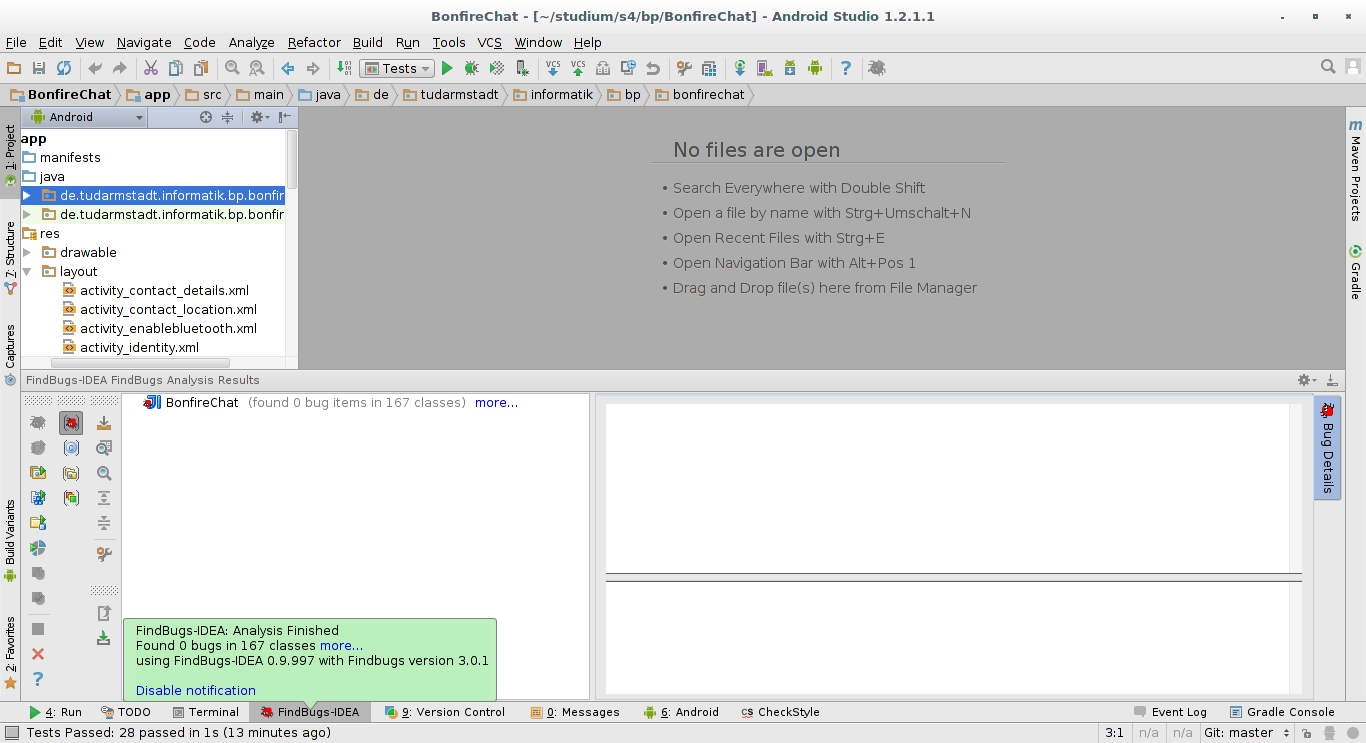
\includegraphics[width=17.5cm]{belege/findbugs/findbugs-no-warnings-screenshot.png}

\subsubsection{Screenshot von FindBugs-IDEA}

Im gezeigten Screenshot ist sichtbar, dass FindBugs eine Stelle im Code markiert hat, an der möglicherweise eine NullPointerException auftreten könnte. Weitere gefundene Fehler sind in der FindBugs-Ansicht unten am Bildschirm erkennbar.

Da betroffene Stellen orange unterstrichen werden und mit einer Fehlermarkierung am Rand angezeigt werden, sind sie direkt bei der Entwicklung der Anwendung ersichtlich und können umgehend behoben werden.

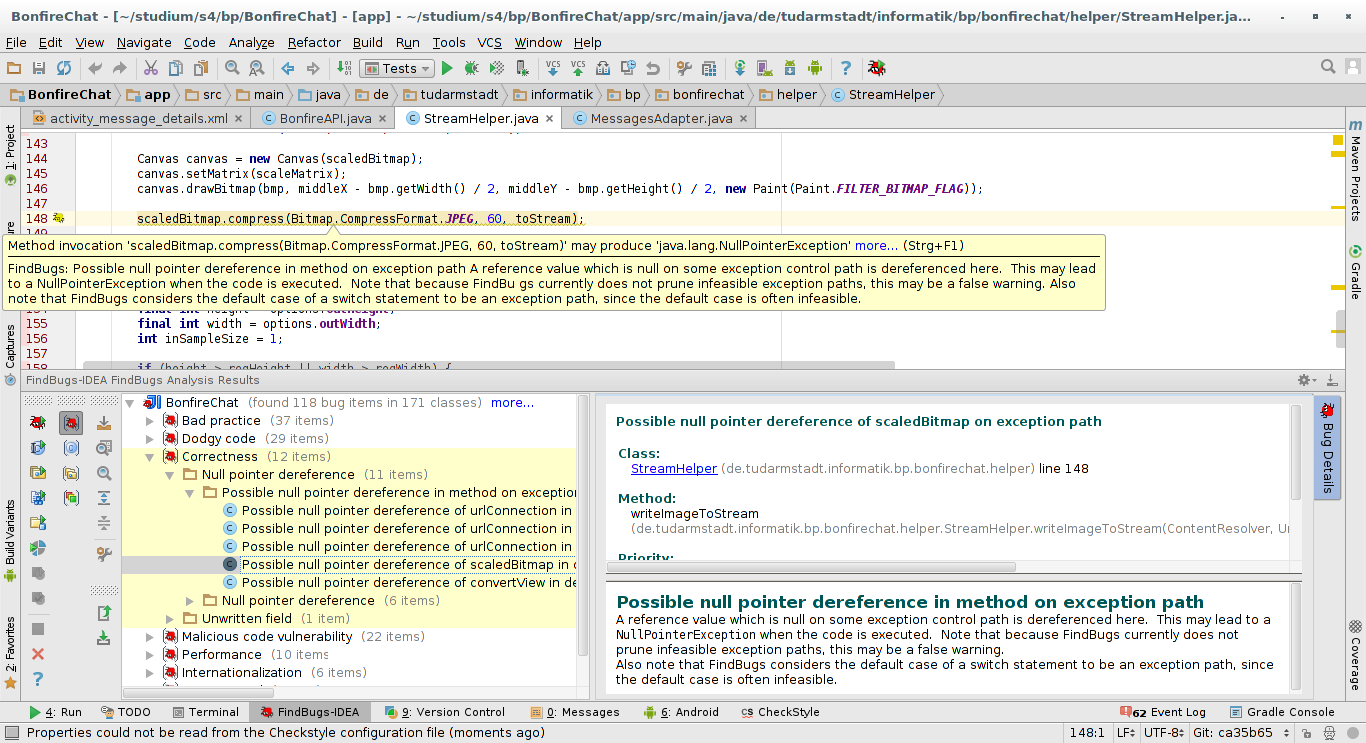
\includegraphics[width=17.5cm]{belege/findbugs/findbugs-idea-screenshot.png}
